\documentclass[11pt]{article}
\usepackage[margin=1in]{geometry}
\usepackage[utf8]{inputenc}
\usepackage[T1]{fontenc}
\usepackage{hyperref}
\hypersetup{colorlinks=true, linkcolor=blue, citecolor=blue, urlcolor=blue,
  pdftitle={Look When Unsure, Check When Sure}, pdfauthor={Caio Vicentino}}
\emergencystretch=3em \sloppy \hyphenpenalty=2000 \exhyphenpenalty=0 \hbadness=10000
\usepackage{booktabs}\usepackage{amsfonts}\usepackage{amsmath}\usepackage{amssymb}
\usepackage{xcolor}\usepackage{array}\usepackage{graphicx}\usepackage{multirow}
\usepackage{tikz}\usetikzlibrary{arrows.meta,positioning,calc,shapes.geometric}
\newcommand{\PENDING}[1]{\textcolor{red}{[#1]}}
\newcommand{\prereg}{\textsc{pre-registered}}
\newcommand{\explo}{\textsc{exploratory}}

\title{Look When Unsure, Check When Sure\\[4pt]
\large Consequence training makes a world model's remaining errors confident---\\
most of all where it knows the world best}
\author{%
  Caio Vicentino \\ OpenInterpretability \\ Fortaleza, Brazil \\
  ORCID: 0009-0003-4331-6259 \\ \texttt{caio@openinterp.org}}
\date{October 2026\\[2pt]
  {\small DOI: \href{https://doi.org/10.5281/zenodo.23146971}{\texttt{10.5281/zenodo.23146971}}}}

\begin{document}
\maketitle

\begin{abstract}
An agent that can predict the consequences of its actions can chain those predictions and plan without acting, but
errors compound, and checking the real state (a \texttt{git status}, a sensor read) costs time. We ask when such an
agent should look, with V42, the first release candidate of Ekbasis, an open 27B consequence model that reads the
probability of every candidate next state from a single forward pass. A simple rule---look when the chain's confidence since the last look falls below 0.9,
plus scheduled checks with a Trickle-style backoff---keeps 197 of 200 fresh 100- and 200-action chains exact in four
worlds, two of them never seen in training, at 17.9 looks per 100 actions; never looking keeps 25 of 40 exact. The
checks are needed because of a pre-registered finding about the model's confidence. On 15,008 new questions, 58.1\% of
its errors in the world families it was trained on carry confidence $\ge 0.9$, against 27.8\% in families it never saw
($+30.3$ points, 95\% CI $[24.0, 36.5]$). The same questions answered by the model \emph{before} consequence training
show almost none (1.9\% and 0.5\%). Training cut its errors in the trained families by two-thirds, but multiplied
confident errors per answer tenfold (0.28 to 2.79 per 100), and further training raised them again.
In long chains, the parent's step probabilities never reach 0.9, right or wrong, so the same rule has to look at 99
of every 100 actions: consequence training is what makes the loop cheap, and what makes the checks necessary.
Pre-registered fixes that reshape confidence---temperature, Platt
and isotonic recalibration, label smoothing, focal loss---fail. Training on the model's own errors made from true
states makes single answers honest, but the loop then looks 81\% more. What fixes the loop is mining errors where they
happen, inside the model's own chains (DAgger-style): on fresh chains this cuts silent wrong steps by 71--97\% with no
more looks. Every such fine-tune, though, failed a pre-registered release criterion, most of them the gate of the git
guard that ships with the model, by forgetting rare work-losing commands such as \texttt{git reset --merge}. An exact
weight interpolation halfway back to V42 passes every single-question and guard criterion, and on 160
fresh chains it keeps the loop's gain: 91\% fewer silent wrong steps with 6\% fewer looks. It then passes the
pre-registered release evaluation, with the guard judged on the larger set, and is released as Ekbasis-27B, with the
checks kept in its default rule. Model, client, data, analysis
code and every pre-registration are open.
\end{abstract}

\section{Introduction}
Agents act in worlds whose state they rarely see in full. Before running \texttt{git checkout -- app.py}, a coding agent
would like to know whether the command throws away uncommitted work; before a long plan, it would like to know where
the plan leaves the world. A \emph{consequence model} (a world model in LeCun's sense \cite{lecun2022}, or a forward
model in Wolpert's \cite{wolpert1995}) answers such questions about the next state given an action. Chained, its
predictions let an agent plan without acting. The price is compounding error: a wrong prediction becomes the premise of
the next one \cite{talvitie2014,janner2019}. Looking at the real state fixes the chain, but every look costs a tool
call, a sensor read or a round trip. When should the agent look?

The classical answer is to predict, observe and correct \cite{kalman1960}, and to observe when the predictor's own
uncertainty crosses a threshold \cite{trimpe2014,holt2023}. We apply it to a language world model, V42, the first release candidate of Ekbasis-27B,
which reads the probability of every answer from one forward pass, with no generation. The chain's confidence is then the
product of those probabilities since the last look, and the agent looks when it drops. On long chains in four worlds,
this works (\S\ref{sec:loop}). The interesting part is \emph{where it fails}, and why.

The model's rare errors in the worlds it knows best are confident. A confidence trigger cannot see them, so the default
rule adds scheduled checks whose interval doubles while the forecasts hold, as in the Trickle algorithm
\cite{rfc6206}. A pre-registered test on 15,008 new questions confirms the pattern beyond the chains
(\S\ref{sec:confident}). A second pre-registered test, against the same model before consequence training, shows that
the training made it. Training improved accuracy and, at the same time, made the remaining errors look like right
answers.

We then report, in the order we ran them, the attempts to make the model's confidence honest:
\begin{itemize}
  \item post-hoc recalibration, training losses and training on the model's own errors made from true states, which
  all fail in the loop (\S\ref{sec:nulls});
  \item mining errors inside the model's own chains, which works, and what it costs (\S\ref{sec:dagger}).
\end{itemize}
Every test was pre-registered \cite{nosek2018}, with its plan's SHA-256 sealed before the run
(Appendix~\ref{app:prereg}), unless marked \explo.

\paragraph{Contributions.}
\begin{itemize}
  \item \textbf{A look-when-unsure loop for a one-pass language world model}, with scheduled checks. It keeps 197 of 200
  fresh long chains exact at 17.9 looks per 100 actions, and it looks 2--9$\times$ more in worlds the model never saw.
  It is the default of the released client.
  \item \textbf{Confident errors where the model was trained} (\prereg): 58.1\% of errors at $\ge 0.9$ in trained
  families against 27.8\% in unseen ones. The ranking of confidences is similar (AUROC 0.92 and 0.91), but the scale
  is not.
  \item \textbf{Training made it} (\prereg, against the parent model): the difference in gaps is $+28.9$ points
  $[22.8, 34.9]$. Confident errors per answer grew tenfold in trained families while total errors fell by two-thirds.
  In long chains the parent never reaches 0.9 and has to look at 99 of every 100 actions.
  \item \textbf{What does not fix it} (\prereg): recalibration, label smoothing and focal loss lower the scale but keep
  the gap, or blur the ranking. Errors mined from true states make single answers honest and the loop look more.
  \item \textbf{What does, and its cost} (\prereg): errors mined inside the model's own chains cut silent wrong steps
  in the loop by 71--97\% on fresh chains. Every such fine-tune failed a release criterion, most of them the git guard's,
  by forgetting rare commands. Halfway back in weight space, the guard holds and the loop keeps its gain (91\% fewer
  silent wrong steps on fresh chains).
\end{itemize}

\section{Setting}\label{sec:setting}
\paragraph{Model.} V42 is Eikos-27B, a decision model fine-tuned from Qwen3.8-27B \cite{qwen38,eikos}, further trained
with LoRA adapters \cite{hu2022} on consequence questions and merged. It was the first release candidate of
Ekbasis-27B; the checkpoint released under that name came out of this work (\S\ref{sec:dagger}). Given rules, a state, one or more actions
and a closed question (yes/no or a choice among listed options), it reads the probability of every option from the
next-token distribution over option letters, in one forward pass, at temperature 1. The consequence questions come from
two sources:
\begin{itemize}
  \item synthetic worlds from seven training families (grids, gravity, counters, lamps, sequences, containers, crafting);
  \item real git repositories: what is in the working tree, the index, the stash and the branches after a command, and
  whether a command fails or loses uncommitted work.
\end{itemize}
The second capability ships as a \emph{git guard}, which asks the model before an agent runs a command. Here it doubles
as a regression gate for any retraining (\S\ref{sec:dagger}). The model before consequence training, Eikos-27B, serves
as the parent in the causal tests.

\paragraph{Worlds and chains.} A chain is 100 or 200 random actions in one of four worlds:
\begin{itemize}
  \item \emph{containers}: 2--3 containers of 3--10 liters, with fill, empty and pour actions;
  \item \emph{lamps}: 4--7 lamps with two or three states and 3--4 buttons, each wired to 1--3 lamps, that advance
  them along their cycle or set them on or off;
  \item \emph{machines}: 3--5 devices that cycle through 3--4 states, with actions that advance all of them, advance
  one or reset one;
  \item \emph{cards}: 4--7 labeled cards in a row, with swaps, segment reversals and shifts.
\end{itemize}
Containers and lamps belong to the training families. Machines and cards were never trained (0 rows in the training
mix).

At each step the model receives the rules, the state it currently believes and one action, and it answers one question
per variable of the state (``How many liters are in A?'') in a single request. The next believed state is the most
probable answer per variable. For cards it is the most probable \emph{valid} permutation, by assignment over the
per-position probabilities \cite{kuhn1955}. The probability of the state read is the product of the chosen answers'
probabilities, and the \emph{chain confidence} $c$ is the product over the steps since the last look.

A \emph{look} returns the exact real state, which replaces the believed one. A step is a \emph{silent wrong step} when
the believed state after it is wrong and no look happened at that step. We report silent wrong steps and looks per
100 actions, and whether the believed state is exactly right after the last action.

\paragraph{Rules.}
\begin{itemize}
  \item \texttt{never}: never look.
  \item \texttt{every 50}: look every 50 actions.
  \item \texttt{step} $\tau$: look when the probability of the state just read is below $\tau$.
  \item \texttt{chain} $\tau$: look when $c<\tau$.
  \item \texttt{until} $\tau$: \texttt{chain} $\tau$, and after a look that finds the forecast wrong (a
  \emph{surprise}), look after every action until a look finds it right.
  \item \texttt{check} $\tau$: \texttt{until} $\tau$ plus scheduled checks. If $g$ actions pass without a look, look.
  The interval $g$ starts at 8, doubles (up to 64) after a look that confirms the forecast, and goes back to 8 after a
  surprise, as in the Trickle algorithm \cite{rfc6206}.
\end{itemize}
No rule looks after the last action. The released client's default is \texttt{check}~0.9 (Figure~\ref{fig:loopdiagram}).

\begin{figure}[t]\centering
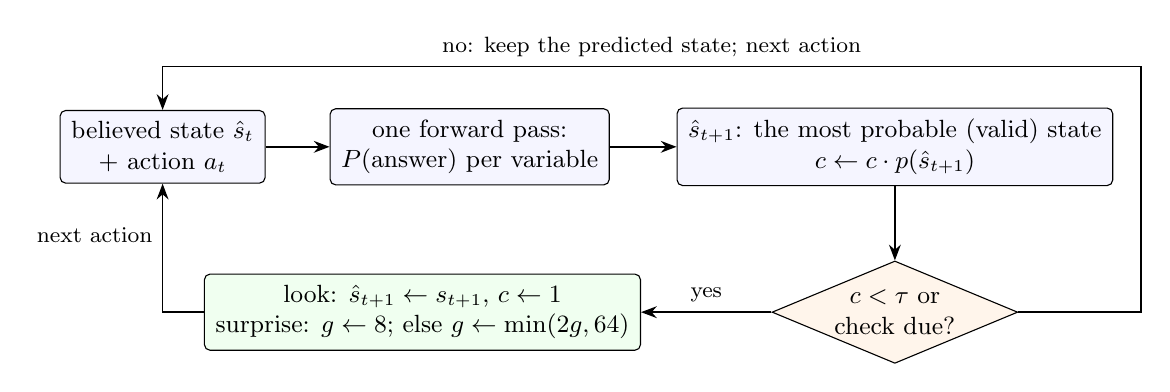
\begin{tikzpicture}[font=\small,
  box/.style={draw, rounded corners=2pt, align=center, inner sep=4pt, fill=blue!4},
  dec/.style={draw, diamond, aspect=2.4, align=center, inner sep=1pt, fill=orange!8},
  look/.style={draw, rounded corners=2pt, align=center, inner sep=4pt, fill=green!6},
  arr/.style={-{Stealth[length=2mm]}, semithick}]
\node[box] (s) at (0,0) {believed state $\hat s_t$\\ + action $a_t$};
\node[box] (p) at (3.9,0) {one forward pass:\\ $P(\text{answer})$ per variable};
\node[box] (r) at (9.3,0) {$\hat s_{t+1}$: the most probable (valid) state\\ $c \leftarrow c \cdot p(\hat s_{t+1})$};
\node[dec] (d) at (9.3,-2.1) {$c<\tau$ or\\ check due?};
\node[look] (l) at (3.3,-2.1) {look: $\hat s_{t+1} \leftarrow s_{t+1}$,\ $c \leftarrow 1$\\ surprise: $g \leftarrow 8$; else $g \leftarrow \min(2g, 64)$};
\draw[arr] (s) -- (p); \draw[arr] (p) -- (r); \draw[arr] (r) -- (d);
\draw[arr] (d) -- node[above, font=\footnotesize] {yes} (l);
\draw[arr] (l.west) -| node[pos=0.8, left, font=\footnotesize] {next action} (s.south);
\draw[arr] (d.east) -- ($(d.east -| r.east)+(0.35,0)$) |- node[pos=0.75, above, font=\footnotesize] {no: keep the predicted state; next action}
  ($(s.north)+(0,0.55)$) -- (s.north);
\end{tikzpicture}
\caption{The loop. The model predicts the next state in one forward pass, and the chain confidence $c$ is the product of
the probabilities of the states read since the last look. The agent looks at the real state when $c$ falls below
$\tau$, or when a scheduled check is due (interval $g$, Trickle-style backoff). The default is $\tau=0.9$.}
\label{fig:loopdiagram}
\end{figure}

\section{Looking when unsure keeps long chains exact}\label{sec:loop}
Table~\ref{tab:rules} compares the rules on the same 40 chains (cards: 8 per length; the other worlds: 4 per length).
This is the \explo{} development set on which the default was chosen. Never looking leaves 24 of 40 chains exact: one
wrong step corrupts every later one, at 32.45 silent wrong steps per 100 actions. Looking every 50 actions does not
help the cards (4 of 16 exact). Confidence-triggered rules keep 39--40 of 40 exact at 9--18 looks per 100 actions.

Two things separate the rules:
\begin{itemize}
  \item \textbf{The trigger must accumulate.} \texttt{step}~0.9 misses errors that build up over several confident
  steps (7 of 8 lamp chains exact); the chain trigger does not.
  \item \textbf{Checks halve the silent wrong steps at a small cost.} \texttt{chain}~0.9 leaves 0.73 silent wrong steps
  per 100 actions, \texttt{check}~0.9 0.40, for 1.4 more looks per 100 actions.
\end{itemize}
Looking again after a surprise until right (\texttt{until}) changes nothing on its own; the checks are what helps, and
\S\ref{sec:confident} shows why.

\begin{table}[t]\centering\small
\caption{Rules compared on the same 40 chains (100 and 200 actions; cards 16, the other worlds 8 each). Silent wrong
steps and looks are per 100 actions. Right: looks per 100 actions by world.}
\label{tab:rules}
\begin{tabular}{lccc|cccc}
\toprule
rule & exact & silent wrong & looks & containers & lamps & machines & cards \\
\midrule
never & 24/40 & 32.45 & 0 & 0 & 0 & 0 & 0 \\
\texttt{step} 0.9 & 39/40 & 2.15 & 12.0 & 1.0 & 0.0 & 1.7 & 28.8 \\
\texttt{chain} 0.5 & 39/40 & 2.82 & 8.7 & 0.2 & 0.2 & 2.1 & 20.5 \\
\texttt{until} 0.5 & 39/40 & 2.55 & 9.6 & 0.3 & 0.2 & 2.1 & 22.7 \\
\texttt{check} 0.5 & 40/40 & 1.30 & 11.1 & 3.2 & 2.9 & 3.7 & 22.8 \\
\texttt{chain} 0.9 & 40/40 & 0.73 & 16.7 & 1.6 & 3.3 & 11.8 & 33.4 \\
\texttt{until} 0.9 & 40/40 & 0.80 & 17.6 & 2.1 & 3.3 & 12.2 & 35.1 \\
\textbf{\texttt{check} 0.9 (default)} & \textbf{40/40} & \textbf{0.40} & \textbf{18.1} & 3.8 & 4.4 & 12.2 & 35.1 \\
\midrule
\multicolumn{8}{l}{\emph{cards only (16 chains)}} \\
\texttt{every 50} & 4/16 & 46.54 & 1.3 & & & & \\
\texttt{chain} 0.9 & 16/16 & 0.00 & 33.4 & & & & \\
two views + \texttt{chain} 0.9 & 16/16 & 0.00 & 17.0 & & & & \\
\bottomrule
\end{tabular}
\end{table}

\paragraph{It looks where it is unsure.} Under the default, the model looks at containers and lamps 3.8 and 4.4 times
per 100 actions, at machines 12.2 and at cards 35.1. The two worlds it never saw get 3--9$\times$ more looks, and all
their chains stay exact. Cards are the hardest: a permutation of 4--7 labels, read position by position. There a
second view helps. Asking also the inverse questions (``At which position is the X?'', a question type the model knows)
and reading both views jointly halves the looks (17.0 against 33.4 per 100 actions), with no error. In an
\explo{} end-to-end check through the released client (4 card chains of 100 actions), the same option cut looks from
44.5 to 27.5 per 100 actions with all chains exact.

\paragraph{Fresh chains.} On 200 chains never used to design the rule (80 card chains, 40 per other world; seeds fixed
in the plans of later pre-registered comparisons), the default keeps 197 of 200 exact, at 0.64 silent wrong steps and
17.9 looks per 100 actions:

\begin{center}\small
\begin{tabular}{lcccc|c}
\toprule
 & containers & lamps & machines & cards & all \\
\midrule
exact & 40/40 & 40/40 & 40/40 & 77/80 & 197/200 \\
silent wrong per 100 actions & 1.68 & 1.48 & 0.00 & 0.03 & 0.64 \\
looks per 100 actions & 4.1 & 4.8 & 10.2 & 35.3 & 17.9 \\
\bottomrule
\end{tabular}
\end{center}

Each of the three misses is a 200-action card chain whose only silent wrong step is the last action, which no rule
looks after. The model had flagged it: the probability of the state read was 0.0005, 0.002 and 0.025. On 40 of these
chains, never looking keeps 25 exact.

\section{Where the errors are confident}\label{sec:confident}
\paragraph{The observation (\explo).} In 40 never-look chains (6,000 steps) we recorded each step's probability and
whether the step itself was right from the model's own previous state:
\begin{itemize}
  \item containers: all 5 wrong steps at probability 0.917--0.988;
  \item lamps: all 4 at 0.991--0.994;
  \item machines: 1 of 3 wrong steps at $\ge 0.9$;
  \item cards: 0 of 82 (the highest 0.626).
\end{itemize}
In the never-seen worlds the model errs often and says so. In the trained worlds it errs rarely and does not. No single
per-step threshold serves all four worlds, and the confidence trigger alone lets the trained worlds' errors through.
The checks catch them: in containers, silent wrong steps go from 2.58 to 1.17 per 100 actions (Table~\ref{tab:rules},
\texttt{chain}~0.9 against \texttt{check}~0.9). Nine errors on the trained side is too few for a claim, and card
orderings differ from the other worlds in kind. So we tested it.

\paragraph{The test (\prereg).} We generated 15,008 new short questions (1--3 actions) from the world generator:
\begin{itemize}
  \item 12 families, 120 per family, question type and number of actions, with seeds never used before;
  \item three groups: \textbf{T}, the 7 training families with their trained question types (7,172); \textbf{H}, the
  same families with a held-out question type (2,472); \textbf{U}, 5 families never trained (5,364).
\end{itemize}
The primary statistic is the share of wrong answers made with confidence $\ge 0.9$, T against U. Its 95\% interval
comes from a percentile bootstrap that resamples items within each family (2,000 resamples) \cite{efron1979}.

\begin{table}[t]\centering\small
\caption{Confident errors on 15,008 new questions (\prereg), for V42 and for the same model before consequence
training (Eikos-27B, the parent), on the same items through the same service at temperature 1. T: trained
families; H: trained families, held-out question types; U: families never trained.}
\label{tab:ce}
\resizebox{\textwidth}{!}{%
\begin{tabular}{llcccccc}
\toprule
 & & n & wrong & errors at $\ge 0.9$ & confident errors & median confidence & AUROC \\
 & & & (\% of answers) & (\% of errors) & per 100 answers & of the errors & \\
\midrule
\multirow{3}{*}{V42} & T & 7,172 & 4.8 & \textbf{58.1} & 2.79 & 0.936 & 0.922 \\
 & H & 2,472 & 13.5 & 37.1 & 5.02 & 0.791 & 0.888 \\
 & U & 5,364 & 14.9 & \textbf{27.8} & 4.14 & 0.748 & 0.908 \\
\midrule
\multirow{3}{*}{Eikos-27B (before)} & T & 7,172 & 14.4 & 1.9 & 0.28 & 0.568 & 0.901 \\
 & H & 2,472 & 35.2 & 0.7 & 0.24 & 0.467 & 0.924 \\
 & U & 5,364 & 21.3 & 0.5 & 0.11 & 0.539 & 0.900 \\
\bottomrule
\end{tabular}}
\end{table}

Confirmed (Table~\ref{tab:ce}, Figure~\ref{fig:ce}). 58.1\% of the errors in T carry confidence $\ge 0.9$, against
27.8\% in U: $+30.3$ points, 95\% CI $[24.0, 36.5]$. The family medians agree (60.9\% against 25.8\%). Among answers that
the actions change (secondary), the gap is larger: 62.0\% against 21.6\%, $+40.4$ $[32.8, 48.1]$. H lies in between
(37.1\%).

The AUROC of confidence for right against wrong answers is similar in T and U (0.922 and 0.908): the model \emph{ranks}
its answers about as well in both groups, but the \emph{scale} differs. One consequence matters for agents. A trigger at
0.9 can flag at most 41.9\% of the errors in T, against 72.2\% in U. Per answer, though, U still has more confident
errors (4.14 against 2.79 per 100), because it has three times as many errors.

\paragraph{Robustness (\explo).}
\begin{itemize}
  \item The pattern holds for yes/no questions (61.3\% against 41.2\%) and choices (55.6\% against 19.9\%).
  \item It holds in every difficulty stratum.
  \item It holds when any single family is left out (gap 22.2--33.5 points).
\end{itemize}
A logistic regression on the wrong answers gives familiarity an odds ratio of 2.44, controlling for the cell's error
rate and the answer format. With families as the unit (a family-cluster bootstrap), however, the interval includes
zero ($[-0.35, 1.63]$ on the log-odds), because two families go against the trend: timers (U, 61.8\%) and counters (T,
32.4\%). It is a strong tendency across items, not a law across families.

\begin{figure}[t]\centering
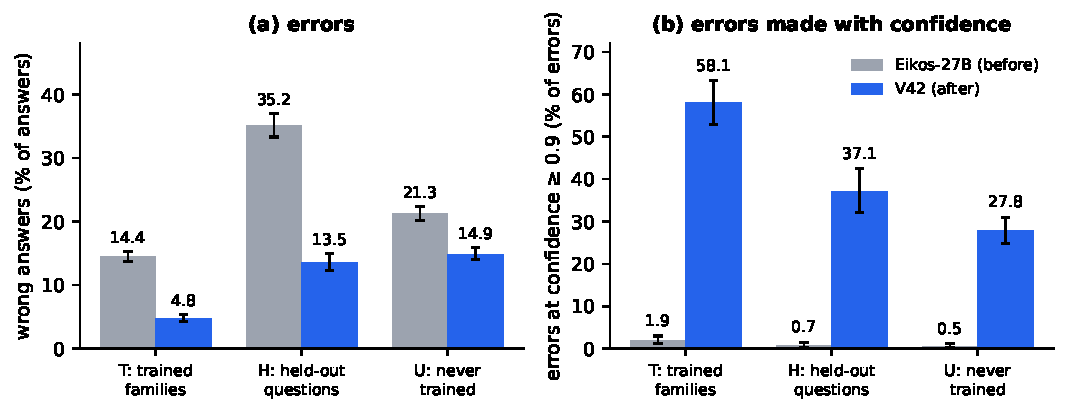
\includegraphics[width=\textwidth]{figures/fig_confident_errors.pdf}
\caption{Consequence training cut errors (a) and made the remaining ones confident (b), most of all in the families it
trained on. The same 15,008 questions, the parent model (Eikos-27B) and V42. Error bars:
Wilson 95\% intervals, for display; the tests use the pre-registered bootstraps.}
\label{fig:ce}
\end{figure}

\paragraph{Training made it (\prereg).} Was the gap there before consequence training, for instance because the
unseen families are simply harder? We asked the parent model, Eikos-27B, the same 15,008 questions through the same
service, letter readout and temperature. Its errors are frequent but almost never confident: 1.9\% of its errors in T
and 0.5\% in U are at $\ge 0.9$ (gap $+1.4$, $[0.4, 2.4]$). Its confidence never exceeds 0.976, a ceiling of its letter
readout, but 0.9 sits inside its range: 54.7\% of its right answers reach it, against 92.6\% of V42's. The pre-registered statistic, the difference between the
two models' gaps by a paired bootstrap, is $D = +28.9$ points, $[22.8, 34.9]$. The training made the gap.

What the training did is visible in Table~\ref{tab:ce}:
\begin{itemize}
  \item it cut errors by two-thirds in T (14.4\% to 4.8\%) and by under a third in U (21.3\% to 14.9\%);
  \item it raised the share of confident errors by 56.2 points in T $[50.8, 61.5]$ and 27.3 in U $[24.3, 30.4]$;
  \item per answer, confident errors went from 0.28 to 2.79 per 100 in T, and from 0.11 to 4.14 in U.
\end{itemize}
On each model's own scale (\explo; the threshold at the confidence of its 10th-percentile right answer: 0.608 for the
parent, 0.943 for V42), the parent already shows a small gap in the same direction ($+8.8$ points)
against $+28.3$ after training. Familiar worlds were slightly more prone to confident errors from the start, and the
training amplified it and lifted the whole scale.

\paragraph{More training, more of it (\explo).} The control arm of our first repair round (\S\ref{sec:nulls})
continued V42's recipe for 200 more steps. It raised the share of confident errors further, from 57.7\% to
67.3\% in T and from 27.1\% to 36.0\% in U (the trainer's own readout), without improving accuracy. Guo et al.\
\cite{guo2017} saw networks grow overconfident late in training, as they overfit the log-likelihood while their
classification error still fell. Here it grows where the model has seen the most.

\paragraph{In the loop (\prereg).} We ran the parent on the 40 chains of Table~\ref{tab:rules}, with every rule
(Figure~\ref{fig:parent}).
\begin{itemize}
  \item \textbf{The prediction holds.} In its never-look traces of the two worlds V42 trained on, 0 of the
  parent's 281 wrong steps reached 0.9, against all 9 of V42's (one-sided Fisher $p = 2.8\times10^{-17}$).
  \item \textbf{It holds for a simpler reason than on single questions.} The parent's step probabilities never reach 0.9
  at all, right or wrong; its highest is 0.8755. A step's probability is the product of several answers, each below
  0.976. They still rank its right steps above its wrong ones (AUROC 0.961 in the trained worlds, 0.914 in the unseen
  ones).
  \item \textbf{It looks at almost every action.} The parent is wrong 31 times as often per step in the trained worlds
  (11.7\% against 0.375\%). It runs the loop with 99.3 looks per 100 actions at chain confidence 0.9 and 51.5 at 0.5,
  against 16.7 and 8.7 for V42.
  \item \textbf{Its checks add nothing}: 0.07 and 0.08 silent wrong steps per 100 actions, without and with them. V42's checks halve its silent wrong steps.
  \item \textbf{Its misses are flagged.} It ends 35 or 36 of 40 chains exact at 0.9. Each of the 9 chains that end wrong
  missed only its last action, which no rule looks after, at a probability of at most 0.38.
\end{itemize}
Consequence training is what makes the loop cheap, and what makes the checks necessary.

\begin{figure}[t]\centering
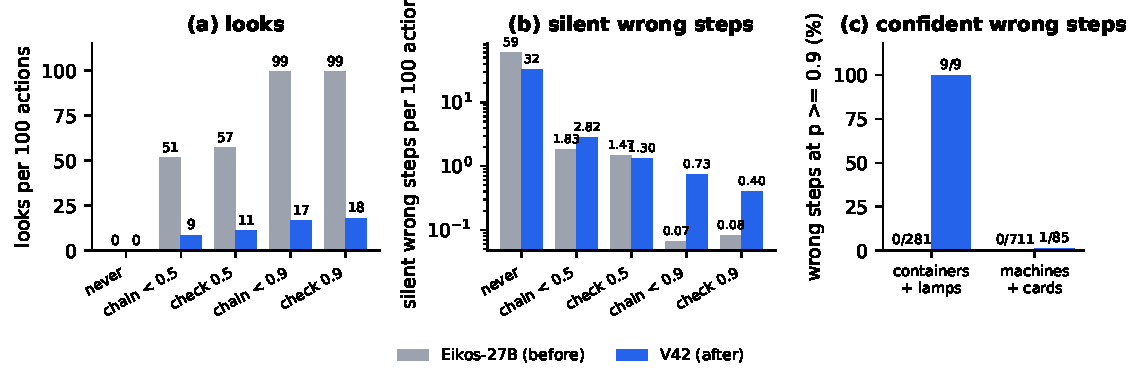
\includegraphics[width=\textwidth]{figures/fig_parent_loop.pdf}
\caption{The same 40 chains before and after consequence training (\prereg). (a) Looks and (b) silent wrong steps per
100 actions under each rule. (c) The share of the never-look traces' wrong steps made at step probability $\ge 0.9$,
with the counts above the bars. The parent errs far more often but never with confidence, so it looks at nearly every
action. V42 looks at fewer than a fifth as many and needs the checks for its confident errors.}
\label{fig:parent}
\end{figure}

\section{What does not fix it}\label{sec:nulls}
\paragraph{Post-hoc recalibration (\prereg).} We fit four maps on 4,998 new items (seeds never used; 40 per family,
question type and number of actions) plus the git validation split (774):
\begin{itemize}
  \item M1, a global temperature;
  \item M2, a temperature from features of the question;
  \item M3, Platt scaling of the chosen answer's confidence \cite{platt1999};
  \item M4, isotonic regression \cite{zadrozny2002}.
\end{itemize}
We then tested them on the 15,008 questions and the git splits (Table~\ref{tab:nulls}, top).
\begin{itemize}
  \item \textbf{The band becomes honest.} The 0.9--0.99 band, which says 96.7\% but is right 84.0\% of the time at
  $T{=}1$, is right 96.8--97.1\% after any map. ECE \cite{naeini2015} falls from 0.049 to 0.010--0.027.
  \item \textbf{The gap stays.} The share of errors at $\ge 0.9$ falls in T and in U alike (T 59.1\% to 24--32\%, U
  27.7\% to 6--10\%), so the T--U gap remains (18--22 points): a map from confidence to confidence cannot tell a
  familiar confident error from a familiar right answer.
  \item \textbf{The guard fails.} Every map raised the guard's false alarms on unseen git commands beyond the
  pre-registered margin (2.4\% to 4.8\%; 11.9\% for isotonic).
\end{itemize}
None was adopted.

\paragraph{Training losses (\prereg).} From the V42 adapter, 200 more steps of V42's recipe with:
\begin{itemize}
  \item cross-entropy (the control);
  \item label smoothing 0.1 \cite{szegedy2016,muller2019};
  \item focal loss with $\gamma{=}2$ \cite{lin2017,mukhoti2020}.
\end{itemize}
Label smoothing cut the confident share to 26.8\% / 14.7\% (T/U) but lowered the AUROC from 0.919 to 0.871. Focal loss
cut it to 9.3\% / 1.5\% with accuracy kept, but lowered the AUROC to 0.891 and became under-confident: its 0.9--0.99
band said 94.2\% and was right 99.1\% of the time. Losses that only lower the scale blur the ranking a trigger depends on.

\paragraph{Training on its own errors, made from true states (\prereg).} V42 answered 47,758 new
questions from the 7 trained families and was wrong on 2,486 (5.2\%), 1,381 of them at $\ge 0.9$.
\begin{itemize}
  \item \textbf{r2err}, trained on those errors (30\% of every batch, 300 steps), made single answers honest. Confident
  errors per 100 answers fell from 2.76 to 0.22 in T ($-92\%$), and also in the held-out types and the never-trained
  families, which were never mined (H 4.81 to 0.44, U 4.03 to 0.56). The AUROC rose from 0.919 to 0.928.
  \item In the loop, on the same 40 chains, r2err looked 81\% more (32.8 against 18.1 per 100 actions): it had become
  unsure where it was right. Right answers at $\ge 0.99$ fell from 74.4\% to 44.1\%.
  \item \textbf{r3w20} (\S\ref{sec:dagger}, Table~\ref{tab:runs}) mixed in right-but-unsure answers (2,486 errors and
  4,972 right answers below 0.99, 20\% of every batch). It beat V42 on the 15,008 questions (accuracy
  90.5\% against 90.2\%; 1.37 confident errors per 100 answers in T against 2.76) and kept most of its sharpness
  (68.0\% of right answers at $\ge 0.99$, against 74.4\%). In the loop, on 240 paired chains, it was not better: 0.50 against 0.42 silent
  wrong steps and 23.1 against 18.9 looks per 100 actions. In the trained worlds' never-look traces, 16 of its 23 wrong
  steps (in 4,800 steps) were confident, against 11 of 13 (in 2,400) for V42.
\end{itemize}
The errors a model makes from true states are not the errors it makes in a chain, where it reads states it predicted
itself. This is the exposure problem of sequence prediction \cite{bengio2015,ranzato2016}, and the reason DAgger trains
on the learner's own distribution \cite{ross2011}.

\paragraph{Changing the loop instead (\prereg).} Without training, on the 40 chains of Table~\ref{tab:rules}:
\begin{itemize}
  \item looking also after the last action: 0.50 silent wrong steps and 18.2 looks, against 0.40 and 18.1;
  \item a threshold that adapts to surprises: 1.03 and 13.1, with 39 of 40 exact;
  \item a second view of each state (``is A full?'', ``are lamps 1 and 2 in the same state?'') that triggers a look
  when it disagrees: 0.17 and 26.5 (silent wrong steps $-58\%$, looks $+46\%$);
  \item only confident disagreements: 0.23 and 25.1;
  \item fusing the two views into one read, by exact Viterbi/forward over the neighbors: 0.82 and 16.4;
  \item partial looks at the least sure variables only (containers, lamps and machines, 24 chains): 1.17 silent wrong
  steps against 0.67, for 13\% fewer variables seen.
\end{itemize}
None improved the default. A second view helps only when it is as reliable as the first and its errors are independent,
which is the case of the cards' inverse questions (\S\ref{sec:loop}) and not of the derived ``same state?'' questions.
A whole look also corrects, in passing, the confident errors of variables the trigger did not suspect, and a partial
look gives that up.

\begin{table}[t]\centering\small
\caption{What did not fix it: post-hoc recalibration (\prereg; V42's answers, fit on separate items)
and training losses (\prereg; 200 more steps from the V42 adapter, the trainer's readout). ``Errors at
$\ge 0.9$'': share of the errors, T / U.}
\label{tab:nulls}
\resizebox{\textwidth}{!}{%
\begin{tabular}{lcccc}
\toprule
recalibration & ECE & 0.9--0.99 band right & errors at $\ge 0.9$ (T / U) & guard false alarms (unseen git) \\
\midrule
none ($T{=}1$) & 0.049 & 84.0\% & 59.1 / 27.7 & 2.4\% \\
M1 global temperature & 0.027 & 96.8\% & 31.9 / 10.4 & 4.8\% \\
M2 temperature from features & 0.027 & 97.0\% & 29.8 / 9.9 & 4.8\% \\
M3 Platt & 0.019 & 97.1\% & 27.5 / 7.6 & 4.8\% \\
M4 isotonic & 0.010 & 97.0\% & 24.3 / 6.4 & 11.9\% \\
\midrule
training loss & AUROC & error in T & errors at $\ge 0.9$ (T / U) & \\
\midrule
V42 & 0.919 & 4.78\% & 57.7 / 27.1 & \\
cross-entropy, 200 more steps (control) & 0.916 & 5.41\% & 67.3 / 36.0 & \\
label smoothing 0.1 & 0.871 & 5.09\% & 26.8 / 14.7 & \\
focal loss, $\gamma{=}2$ & 0.891 & 4.67\% & 9.3 / 1.5 & \\
\bottomrule
\end{tabular}}
\end{table}

\section{Mining errors where they happen, and what it costs}\label{sec:dagger}
\paragraph{Chain mining.} V42 ran 200 new chains in the two trained worlds (containers and lamps; seeds
used by no test), never looking. At every step, each variable it answered wrong, or right below 0.99, was saved with
the true result of the action \emph{from the state it was reading}, its own prediction. This gave 555 items (134 wrong,
421 right but unsure). Machines and cards were never mined. The idea is DAgger's \cite{ross2011}, and Data as
Demonstrator's for multi-step prediction \cite{venkatraman2015}: train on the states the model itself visits. The runs
are in Table~\ref{tab:runs}.

\begin{table}[t]\centering\small
\caption{Training on its own errors. Single questions: the trainer's readout on the 15,008 items (accuracy; confident
errors per 100 answers in T / H / U). Loop: the default rule on chains paired with V42, silent wrong steps
and looks per 100 actions. Guard: the pre-registered gate on the larger guard set (Table~\ref{tab:guard}).}
\label{tab:runs}
\resizebox{\textwidth}{!}{%
\begin{tabular}{p{5.6cm}cccc}
\toprule
run (from V42) & accuracy & confident errors & loop: silent wrong, looks & guard gate \\
\midrule
V42 & 90.2 & 2.76 / 4.81 / 4.03 & --- & --- \\
r2err: errors from true states (30\%) & 89.4 & 0.22 / 0.44 / 0.56 & 0.40$\to$0.02, 18.1$\to$32.8 & not run \\
r3w20: errors + unsure answers from true states (20\%) & 90.5 & 1.37 / 2.39 / 3.00 & 0.42$\to$0.50, 18.9$\to$23.1 & not run \\
\textbf{r4a}: errors + unsure (20\%) + chain items (10\%) & 90.7 & 1.70 / 3.20 / 3.37 & \textbf{0.93$\to$0.03}, 18.6$\to$18.2 & fails (recall) \\
\textbf{r4b}: r3w20, then errors + unsure (10\%) + chain items (15\%) & 90.8 & 1.85 / 4.05 / 4.23 & \textbf{0.93$\to$0.09}, 18.6$\to$15.0 & fails (recall) \\
\textbf{r4c}: chain items only (20\%) & 90.3 & 2.34 / 4.49 / 4.25 & \textbf{0.45$\to$0.13}, 16.4$\to$12.9 & fails (alarms) \\
r5a--c: chain items, git share of every batch kept & 89.8--91.0 & 1.92--3.03 (T) & not run & 2 of 3 fail \\
\midrule
\textbf{w4a5}: halfway between V42 and r4a & 90.7 & 2.05 / 3.84 / 3.67 & \textbf{0.57$\to$0.05}, 16.7$\to$15.7 & passes \\
\bottomrule
\end{tabular}}
\end{table}

\paragraph{It fixes the loop.} An \explo{} test on the 240 chains of the earlier loop tests came first: silent wrong
steps fell from 0.42 to 0.07 (r4a) and 0.13 (r4b) per 100 actions, at 18.7 and 15.1 looks against 18.9. A
pre-registered confirmation on 160 fresh chains then confirmed both (Figure~\ref{fig:loop}b):
\begin{itemize}
  \item r4a: silent wrong steps 0.93 to 0.03 per 100 actions ($-97\%$), looks 18.6 to 18.2;
  \item r4b: 0.93 to 0.09 ($-90\%$), looks 15.0 ($-19\%$), with 79 exact chains against 77 of 80.
\end{itemize}
The gains reach the worlds that were never mined. In machines, looks fell from 9.6 to 4.5 (r4a) and 3.5 (r4b) per 100
actions with no wrong step, and r4b kept 31 of 32 card chains exact against 29. Lamps went from 3.04 silent wrong steps
per 100 actions to none in both runs.

r4c, trained on the chain items alone, was confirmed on another 160 fresh chains: 0.45 to 0.13 ($-71\%$), looks 16.4 to
12.9 ($-21\%$), 80 of 80 exact. Training on errors from true states pushed the loop toward more looks, while chain
mining moved it to fewer silent errors at the same or lower cost (Figure~\ref{fig:loop}b).

\begin{figure}[t]\centering
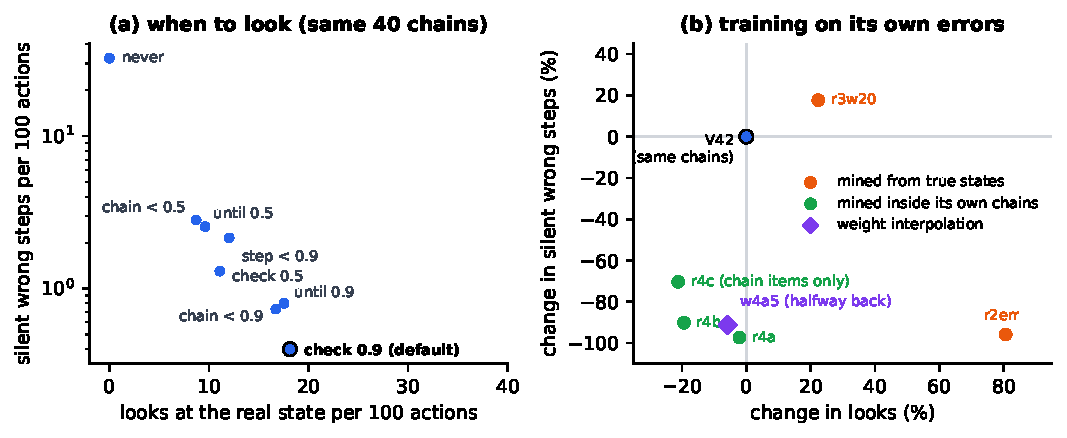
\includegraphics[width=\textwidth]{figures/fig_loop.pdf}
\caption{(a) The rules of Table~\ref{tab:rules} on the same 40 chains (V42); the default is circled.
(b) Training on the model's own errors, against V42 on the same chains (default rule): errors mined from
true states (orange) buy honesty with looks; errors mined inside the model's own chains (green) cut silent wrong steps
with no more looks; the weight interpolation (purple) keeps that gain. r2err: 40 chains; r3w20: 240; r4a and r4b: 160
fresh; r4c and w4a5: another 160 fresh each.}
\label{fig:loop}
\end{figure}

\paragraph{It costs rare knowledge.} A release candidate must also pass the git guard's pre-registered gate:
\begin{itemize}
  \item work-losing commands flagged at $p \ge 0.2$, and false alarms on safe ones, on unseen repositories;
  \item each within one point of V42, on a split of known command types and one of command types held out
  of training.
\end{itemize}
V42 flags 50 of 51 and 41 of 42 work-losing commands, with 0 of 51 and 1 of 42 false alarms. The results:
\begin{itemize}
  \item r4a flagged 39 of 42 held-out commands (2 of 42 false alarms);
  \item r4b flagged 49 of 51 known and 37 of 42 held-out commands;
  \item r4c flagged all 42 held-out commands, but missed one known command and raised more false alarms (1 of 51
  known, 3 of 42 held-out);
  \item a fifth round kept every batch's git share at V42's, and all three runs still lost two or three
  held-out commands (the trainer's readout: 38, 39 and 38 of 42, against V42's 41).
\end{itemize}
What was lost is specific. r4a stopped flagging two work-losing command sequences and r4b five, five distinct ones in
all. Three of them involve \texttt{git reset --merge}, and both runs missed two of those; the other two are a
\texttt{git stash drop} after a \texttt{stash pop} and a \texttt{git restore --source=HEAD\textasciitilde 1}. Meanwhile the median probability they gave to work-losing commands
\emph{rose} (0.983 to 0.986 and 0.991). This is forgetting of rare cases \cite{kirkpatrick2017,luo2023}, not a shift of
the whole scale.

\paragraph{A larger gate.} On the small sets, one item is worth more than the one-point margin. We therefore
pre-registered a 17$\times$ larger guard set, drawn from repository states that no earlier set contains:
\begin{itemize}
  \item known command types: 863 work-losing and 863 safe commands;
  \item command types held out of training: 799 work-losing and 799 safe commands.
\end{itemize}
It replaced the small sets as the gate, with the same rule of one point per split, and every model was scored by the
trainer's readout (Table~\ref{tab:guard}). That readout matches the served model: through vLLM and the API, the release
model flags 827 and 771 work-losing commands and raises 50 and 54 false alarms, and it makes the same flag decision as
the readout on 3,321 of the 3,324 items.
\begin{itemize}
  \item Three of the six chain-mined runs lose work-losing commands beyond the margin on both splits (r4a, r4b and r5c),
  and r5a on the held-out split.
  \item r4c flags slightly more work-losing commands than V42, but raises too many false alarms (59 and
  66 against 50 and 53).
  \item r5b passes the guard, but had already failed another criterion of its round: answers that the actions change in
  multi-step questions, 80.3\% against 81.3\%.
\end{itemize}

\paragraph{Halfway back in weight space.} Interpolating the weights of a fine-tuned model with those of its starting
point can keep most of the gains and recover what was lost \cite{wortsman2022}. With LoRA adapters the interpolation is
exact: the two adapters are concatenated into one of rank 128, with the factors scaled by $\sqrt{1-\lambda}$ and
$\sqrt{\lambda}$, which gives the weights $W_0 + (1-\lambda)\Delta_{\text{release}} + \lambda\Delta_{\text{run}}$. We
pre-registered three interpolations.
\begin{itemize}
  \item \textbf{w4a5}, halfway between V42 and r4a ($\lambda=0.5$), passes every criterion: the guard on
  both splits, every single-question criterion, and confident errors in T not higher (2.05 against 2.76 per 100
  answers). Its accuracy on the 15,008 questions is 90.7\% against 90.2\%, and 74.1\% of its right answers stay at
  $\ge 0.99$, against 74.4\%.
  \item w4a7 ($\lambda=0.7$ toward r4a) and w4b5 (halfway toward r4b) lose too many known work-losing commands.
\end{itemize}
\paragraph{In the loop (\prereg).} w4a5 then ran on 160 chains that no model or test had used (cards seeds 48--63, the
other worlds 24--31), paired with V42, under round 4's confirmation criteria. It is confirmed:
\begin{itemize}
  \item silent wrong steps 0.57 to 0.05 per 100 actions ($-91\%$), looks 16.7 to 15.7 ($-6\%$), and 79 of 80 chains exact
  for both;
  \item in containers, where V42's confident errors concentrate, 2.79 to 0.21 silent wrong steps per 100
  actions;
  \item in machines, never mined, looks 9.9 to 6.8.
\end{itemize}
Interpolating halfway back kept nearly all of r4a's gain in the loop and none of its losses on the guard.

\paragraph{Release evaluation (\prereg).} On the exact merged weights, served:
\begin{itemize}
  \item every non-guard criterion passes: git3 96.62\% of all questions against 96.39\%; answers that the actions
  change in multi-step questions 81.16\% against 81.16\% (78.03\% against 78.20\% read once); the never-trained
  families' changed answers 81.88\% against 81.72\%; ECE 0.024 against 0.027;
  \item the 16 fresh real-repository scenarios are identical: 3 of 3 work-losing flagged, 1 false alarm of 13;
  \item on the small git sets it flags 40 of the 42 held-out work-losing commands, against 41. The original gate would
  fail it by that one item;
  \item under the gate that replaced it (\texttt{PLAN\_guard\_set.md}), it passes. Served on the larger set, it flags 828
  and 767 work-losing commands (against 827 and 771) and raises 37 and 49 false alarms (against 50 and 54);
  \item on the real-use test, rerun on the two repositories' later state (72 new scenarios, 28 work-losing), it and V42 answer alike: 28 of 28 flagged, no false alarm, 92 of 96 ``will it fail?'' right;
  \item under the injection secondary, one more borderline answer crossed 0.5: a ``will it fail?'' that the planted
  branch name moved from 0.44 to 0.53 (V42: 0.13 to 0.27). No work-losing command was missed.
\end{itemize}
It is the first candidate to pass every gate.

\begin{table}[t]\centering\small
\caption{The git guard on the larger pre-registered set (\prereg; the trainer's readout). Work-losing commands flagged at
$p \ge 0.2$ and false alarms on safe commands, on known command types (863 + 863) and held-out ones (799 + 799). The gate
is one point per split against V42.}
\label{tab:guard}
\begin{tabular}{lcccc|l}
\toprule
 & \multicolumn{2}{c}{known types} & \multicolumn{2}{c|}{held-out types} & \\
model & flagged & false alarms & flagged & false alarms & gate \\
\midrule
V42 & 829 & 50 & 771 & 53 & --- \\
r4a & 812 & 44 & 763 & 49 & fails \\
r4b & 776 & 27 & 732 & 35 & fails \\
r4c & 832 & 59 & 776 & 66 & fails \\
r5a & 825 & 45 & 758 & 45 & fails \\
r5b & 821 & 33 & 764 & 44 & passes \\
r5c & 820 & 37 & 759 & 30 & fails \\
\midrule
\textbf{w4a5} & 826 & 40 & 768 & 49 & \textbf{passes} \\
w4a7 & 819 & 38 & 769 & 47 & fails \\
w4b5 & 819 & 36 & 766 & 45 & fails \\
\bottomrule
\end{tabular}
\end{table}

\paragraph{Real use (\explo).} We ran 72 scenarios on independent copies of two real repositories in their current
state (remotes pointed at local paths, hooks off). Truth comes from executing each scenario on its copy: 28 scenarios
lose uncommitted work, and 9 contain a command that fails. V42 and r4c gave the same answers:
\begin{itemize}
  \item all 28 work-losing scenarios flagged, with no false alarm on the other 44;
  \item 92 of 96 ``will it fail?'' questions right;
  \item a median of 0.89 s per check.
\end{itemize}
Whatever separates the two models on the generated sets did not show up in these 72 scenarios.

\paragraph{The release decision.} The interpolation was the first candidate to pass every gate, and it is released as
Ekbasis-27B, with \texttt{check}~0.9 kept as the client default: its familiar errors are fewer, not gone. A retraining
of the whole lineage with chain items from the start, where the rare git knowledge is learned alongside them rather than
overwritten, remains the cleaner route.

\section{Discussion}\label{sec:disc}
\paragraph{Why familiar errors are confident.} One reading fits every measurement here, though we did not test it
causally. Consequence training lifts the whole confidence scale.
\begin{itemize}
  \item Before it, 54.7\% of the parent's right answers reach 0.9. After it, 92.6\% do, and 74.4\% reach 0.99 (83.8\%
  in the trained families).
  \item In the worlds the model trained on, its few remaining errors come out of that sharpened distribution and look
  like its right answers.
  \item In worlds it never saw, the scale is lower for right and wrong answers alike (62.4\% of right answers at
  $\ge 0.99$ in U), so more of its errors stay below the trigger.
\end{itemize}
The ranking survives (AUROC 0.922 and 0.908), so what fails is a fixed threshold, not the model's ordering. The chains
say the same: the parent ranks its right steps above its wrong ones about as well as V42 (AUROC 0.961 and
0.946 in the trained worlds), on a scale that never reaches 0.9. Further
training moves in the same direction, and on each model's own scale the gap is larger after training than before
($+28.3$ against $+8.8$ points).

\paragraph{What to do in an agent.}
\begin{itemize}
  \item Trigger looks on the chain's accumulated confidence, not on single steps.
  \item Add scheduled checks with a backoff. Here they cost 1.4 looks per 100 actions and halve the silent wrong steps.
  \item Expect the trigger to fire least where the model is most trusted: the checks are for that part.
  \item Use a second view only if it is as reliable as the first and fails independently, as the cards' inverse
  questions do. Otherwise it buys honesty with looks.
  \item To train the problem away, mine errors on the states the model itself visits.
  \item Gate every retraining on rare cases with a set large enough that one item is not the whole margin.
\end{itemize}

\paragraph{What the next test caught.} Several results that looked like fixes did not survive the next test.
\begin{itemize}
  \item r3w20 beat V42 on the 15,008 questions and not in the loop.
  \item r2hard had no silent wrong step on the 100-action chains (against 0.55 per 100 actions), but on the 200-action
  chains it had as many (0.35 against 0.33), while looking more at both lengths.
  \item The chain-mined runs that won the loop then lost rare git commands.
\end{itemize}
A single test would have reported each of these as a fix. Read together, they show the pattern: the gain follows where
the training data comes from, and something else gives way.

\section{Related work}\label{sec:related}
\paragraph{When to observe.}
\begin{itemize}
  \item \emph{Predict, observe, correct} is Kalman's \cite{kalman1960}.
  \item \emph{Event-triggered sampling and estimation} measure when needed rather than on a clock
  \cite{astrom2002,tabuada2007}.
  \item \emph{Variance-based triggering} measures when the estimator's own uncertainty crosses a threshold, and its
  schedules tend to become periodic \cite{trimpe2014}.
  \item \emph{Active observing in continuous-time control} learns a model that observes when its uncertainty crosses a
  threshold, and shows that regular observation is not optimal \cite{holt2023}.
  \item \emph{Infoprop} tracks the error accumulated along model-based rollouts \cite{infoprop2025}.
  \item \emph{Trickle} gives the backoff our checks use \cite{rfc6206}.
\end{itemize}
Our loop is this principle applied to a language world model whose uncertainty is read from logits in one pass. We add
a measured failure mode of the trigger, confident errors where the model was trained, which is why scheduled checks
belong in the default.

\paragraph{Language agents that consult the world.} FLARE retrieves when a language model is unsure \cite{flare2023};
KnowNo asks for help from multiple-choice likelihoods \cite{knowno2023}. Song and Cai probe the environment and report
that self-reported uncertainty fails under confident wrong beliefs \cite{songcai2026}, which matches what we measure in
the familiar part of the model's world. Language world models predict the consequences of actions for planning:
\begin{itemize}
  \item reasoning as planning with a world model \cite{hao2023};
  \item text-based world simulators \cite{wang2024sim};
  \item web world models \cite{gu2024webdreamer};
  \item Qwen-AgentWorld, which reasons at length before predicting \cite{qwenagentworld}; Ekbasis answers in one pass.
\end{itemize}
In learned-model RL \cite{ha2018,hafner2020,muzero2020}, compounding model error limits rollout length
\cite{talvitie2014,janner2019}. Closest for agents:
\begin{itemize}
  \item Active Epistemic Control queries the environment to verify uncertain facts and uses world-model predictions only
  to prune plans \cite{aec2026};
  \item DreamPhase imagines futures offline and scores them with an uncertainty-aware value \cite{dreamphase2026};
  \item guards that predict the consequence or risk of an agent's action before it runs, on the web \cite{webguard2025} and
  on mobile interfaces, where SeerGuard predicts the next screen \cite{seerguard2026}.
\end{itemize}
Our git guard is of the last kind, and here it also serves as a regression gate.

\paragraph{Calibration and familiarity.}
\begin{itemize}
  \item Modern networks are overconfident \cite{guo2017}, and calibration degrades under dataset shift
  \cite{ovadia2019}.
  \item The maximum softmax probability separates misclassified and out-of-distribution inputs from correct ones
  \cite{hendrycks2017}, and selective prediction builds on it \cite{geifman2017,kamath2020}.
  \item Language models mostly know what they know \cite{kadavath2022}, post-training can hurt calibration \cite{gpt4},
  and how fine-tuning treats unfamiliar examples shapes how models err \cite{kang2024}.
\end{itemize}
Our result sits between these. V42's errors in unfamiliar worlds are frequent and flagged, while its rare
errors in familiar worlds are confident, and the parent model shows that consequence training created the difference.

\paragraph{Training on the learner's own states, and forgetting.}
\begin{itemize}
  \item DAgger \cite{ross2011} and Data as Demonstrator \cite{venkatraman2015} train on the learner's own distribution;
  scheduled sampling \cite{bengio2015} and sequence-level training \cite{ranzato2016} address exposure bias.
  \item Fine-tuning forgets \cite{kirkpatrick2017,luo2023}; weight-space interpolation can trade the gains against the
  losses \cite{wortsman2022}.
\end{itemize}

\section{Limitations}\label{sec:lim}
\begin{itemize}
  \item \textbf{Synthetic chain worlds.} The four chain worlds are synthetic, and a look is exact and costs the same
  every time. The real-repository evidence (the git guard) concerns single commands, where the agent can read
  \texttt{git status} before each one; a long-horizon loop in a real environment is the next test.
  \item \textbf{One model.} We study one model lineage (a 27B hybrid model) and one parent, so whether other
  consequence models show the same familiarity effect is open.
  \item \textbf{Small numbers in the chain observation.} It rests on 9 trained-world errors in the traces. The
  pre-registered tests carry the claim, and at the family level their effect is a tendency (two families go against
  it).
  \item \textbf{The parent's ceiling.} The parent's letter readout never puts more than 0.976 on one option, so a
  fixed threshold compares scales as much as models. The own-scale analysis and the AUROCs address this, but only in
  part.
  \item \textbf{Different readouts.} The trainer's readout (training rounds) and the service's readout (release tests)
  differ slightly, for instance 57.7\% against 58.1\% for V42 in T; each comparison uses one readout on
  both sides.
  \item \textbf{Training data.} The replay data of the lineage came from the parent's training snapshot and included
  about 48 draws of FinQA items, a family the parent uses for evaluation. No evaluation here uses FinQA.
\end{itemize}

\section{Conclusion}
A one-pass consequence model can keep long action chains exact by looking only when its chain confidence drops. It
looks rarely in the worlds it knows and often in those it does not. Its confidence fails in a specific place, though:
where it was trained, its few remaining errors look like its right answers. Training made them so, and more training
makes more of them. Recalibration and smoother losses do not remove them; training on the errors it makes inside its
own chains does, at the price of rare knowledge elsewhere, and an exact interpolation halfway back to V42
keeps the gain without the price. Its familiar errors are fewer, not gone: an agent should still look when unsure and
check when sure.

\section*{Acknowledgments}
This work was done with Claude Opus 5.5 (Anthropic), which helped plan and run the experiments, write the analysis code
and the text, and check every number and reference.

\section*{Reproducibility}
Everything below is open:
\begin{itemize}
  \item the released model, the interpolation (\texttt{caiovicentino1/Ekbasis-27B}, with FP8, INT4 and MLX builds),
  and V42's predictions and chains, the data of this paper (\texttt{results\_v42/} in the code repository);
  \item the client with the loop (\texttt{ekbasis}, \texttt{simulate(observe=...)});
  \item the training data (\texttt{caiovicentino1/ekbasis-data}).
\end{itemize}
The code, with the saved predictions and chains, and the model weights are under Apache-2.0. In the training data, the
generated rows (worlds and git) are under Apache-2.0, and the replayed rows keep their sources' licenses (CC BY 4.0,
ODC-BY or MIT; each row names its own, and the dataset card lists them). This paper is under CC BY 4.0.
The paper folder of the code repository holds:
\begin{itemize}
  \item every analysis script;
  \item \texttt{reproduce.py}, which re-runs each pre-registered analysis on the saved predictions and chains and checks
  that it reproduces the stored result exactly;
  \item \texttt{numbers.json}, with every number cited here, and \texttt{check\_numbers.py}, which checks that every
  number in the text comes from it;
  \item \texttt{make\_figs.py}.
\end{itemize}
Every plan's SHA-256 was sealed before its run (Appendix~\ref{app:prereg}); \texttt{reproduce.py} also checks that every
plan still matches its seal.

\appendix
\section{Pre-registrations}\label{app:prereg}
Each plan was written and its SHA-256 recorded (\texttt{PREREG\_sha256.txt}) before the run it governs. The plans are
published with the code: the \texttt{PREREG} files at the repository root and the \texttt{PLAN} files under
\texttt{paper/prereg/}. Times are BRT (UTC$-3$).

\begin{center}\footnotesize
\begin{tabular}{p{5.6cm}p{4.9cm}p{3.6cm}}
\toprule
plan & what it tests & sealed \\
\midrule
\texttt{PREREG\_confident\_errors.md} & T against U, 15,008 questions & 10-03 18:30, 9644dbbe \\
\texttt{PREREG\_confident\_errors\_eikos.md} & the same on the parent; $D$ & 10-03 18:48, f5d00582 \\
\texttt{PREREG\_recalibration.md} & M1--M4 & 10-03 19:11, 0dede309 \\
\texttt{PLAN\_v43\_calibration.md} & training losses & 10-03 19:11, 9fee0b87 \\
\texttt{PLAN\_v43\_round2.md} & errors from true states & 10-03 19:57, de7b86d0 \\
\texttt{PLAN\_v43\_loop\_test.md} & r2err in the loop & 10-03 21:39, 9d69d449 \\
\texttt{PLAN\_v43\_round3.md} & dose; r3w20 in the loop & 10-03 22:48, 9b1e422e \\
\texttt{PLAN\_loop\_ideas.md}, \texttt{2}, \texttt{3}, \texttt{4} & loop changes without training & 10-04 00:55--03:14 \\
\texttt{PLAN\_v43\_round4.md} & chain mining & 10-04 00:55, f5a43813 \\
\texttt{PLAN\_v43\_round4\_loop\_explore.md} & r4a, r4b on 240 chains (\explo) & 10-04 03:04, 95069db2 \\
\texttt{PLAN\_v43\_round4\_confirm.md}, \texttt{\_r4a.md} & confirmation on 160 fresh chains & 10-04 04:36, 1988728f; 04:38, 5089819e \\
\texttt{PLAN\_v43\_release\_eval.md} & the release gate & 10-04 04:41, 6f98d66a \\
\texttt{PLAN\_v43\_round5.md} & git share kept & 10-04 07:51, a865a3fe \\
\texttt{PLAN\_v43\_r4c\_loop.md} & r4c on 160 fresh chains & 10-04 08:55, 1f7d1809 \\
\texttt{PLAN\_v43\_wise.md}, addendum & weight interpolation & 10-04 08:57, 1f82e2a0; 09:44, 8666e4d0 \\
\texttt{PLAN\_guard\_set.md} & the 17$\times$ larger guard set & 10-04 09:42, 88c71c83 \\
\texttt{PLAN\_paper\_base\_loop.md} & the parent in the loop & 10-04 13:02, 0b4ba207 \\
\bottomrule
\end{tabular}
\end{center}

\begin{thebibliography}{99}\small
\bibitem{astrom2002} K. J. \AA{}str\"{o}m and B. M. Bernhardsson. Comparison of Riemann and Lebesgue Sampling for First Order Stochastic Systems. In Proceedings of the 41st IEEE Conference on Decision and Control (CDC), vol. 2, pp. 2011--2016, 2002. DOI: 10.1109/CDC.2002.1184824.
\bibitem{bengio2015} S. Bengio et al. Scheduled Sampling for Sequence Prediction with Recurrent Neural Networks. In Advances in Neural Information Processing Systems 28 (NIPS), 2015. arXiv:1506.03099.
\bibitem{efron1979} B. Efron. Bootstrap Methods: Another Look at the Jackknife. The Annals of Statistics, 7(1):1--26, 1979. DOI: 10.1214/aos/1176344552.
\bibitem{eikos} C. Vicentino. Eikos-27B (model) and Eikos (code). Hugging Face and GitHub, 2026. \url{https://huggingface.co/caiovicentino1/Eikos-27B}.
\bibitem{flare2023} Z. Jiang et al. Active Retrieval Augmented Generation. In Proceedings of EMNLP, 2023. arXiv:2305.06983.
\bibitem{infoprop2025} B. Frauenknecht et al. On Rollouts in Model-Based Reinforcement Learning. In International Conference on Learning Representations (ICLR), 2025.
\bibitem{geifman2017} Y. Geifman and R. El-Yaniv. Selective Classification for Deep Neural Networks. In Advances in Neural Information Processing Systems 30 (NIPS), 2017. arXiv:1705.08500.
\bibitem{gpt4} OpenAI. GPT-4 Technical Report. arXiv preprint, 2023. arXiv:2303.08774 (Figure 8: post-training hurts calibration).
\bibitem{gu2024webdreamer} Y. Gu et al. Is Your LLM Secretly a World Model of the Internet? Model-Based Planning for Web Agents. Transactions on Machine Learning Research (TMLR), 2025. arXiv:2411.06559.
\bibitem{guo2017} C. Guo et al. On Calibration of Modern Neural Networks. In Proceedings of the 34th International Conference on Machine Learning (ICML), PMLR 70:1321--1330, 2017. arXiv:1706.04599.
\bibitem{ha2018} D. Ha and J. Schmidhuber. Recurrent World Models Facilitate Policy Evolution. In Advances in Neural Information Processing Systems 31 (NeurIPS), 2018. arXiv:1809.01999.
\bibitem{hafner2020} D. Hafner et al. Dream to Control: Learning Behaviors by Latent Imagination. In International Conference on Learning Representations (ICLR), 2020. arXiv:1912.01603.
\bibitem{hao2023} S. Hao et al. Reasoning with Language Model is Planning with World Model. In Proceedings of EMNLP, pp. 8154--8173, 2023. DOI: 10.18653/v1/2023.emnlp-main.507.
\bibitem{hendrycks2017} D. Hendrycks and K. Gimpel. A Baseline for Detecting Misclassified and Out-of-Distribution Examples in Neural Networks. In International Conference on Learning Representations (ICLR), 2017. arXiv:1610.02136.
\bibitem{holt2023} S. Holt, A. H\"{u}y\"{u}k, and M. van der Schaar. Active Observing in Continuous-time Control. In Advances in Neural Information Processing Systems 36 (NeurIPS), 2023.
\bibitem{hu2022} E. J. Hu et al. LoRA: Low-Rank Adaptation of Large Language Models. In International Conference on Learning Representations (ICLR), 2022. arXiv:2106.09685.
\bibitem{janner2019} M. Janner et al. When to Trust Your Model: Model-Based Policy Optimization. In Advances in Neural Information Processing Systems 32 (NeurIPS), 2019. arXiv:1906.08253.
\bibitem{kadavath2022} S. Kadavath et al. Language Models (Mostly) Know What They Know. arXiv preprint, 2022. arXiv:2207.05221.
\bibitem{kalman1960} R. E. Kalman. A New Approach to Linear Filtering and Prediction Problems. Journal of Basic Engineering, 82(1):35--45, 1960. DOI: 10.1115/1.3662552.
\bibitem{kamath2020} A. Kamath, R. Jia, and P. Liang. Selective Question Answering under Domain Shift. In Proceedings of ACL, pp. 5684--5696, 2020. DOI: 10.18653/v1/2020.acl-main.503.
\bibitem{kang2024} K. Kang et al. Unfamiliar Finetuning Examples Control How Language Models Hallucinate. In Proceedings of NAACL (Long Papers), pp. 3600--3612, 2025. DOI: 10.18653/v1/2025.naacl-long.183.
\bibitem{kirkpatrick2017} J. Kirkpatrick et al. Overcoming Catastrophic Forgetting in Neural Networks. Proceedings of the National Academy of Sciences, 114(13):3521--3526, 2017. DOI: 10.1073/pnas.1611835114.
\bibitem{knowno2023} A. Z. Ren et al. Robots That Ask For Help: Uncertainty Alignment for Large Language Model Planners. In Conference on Robot Learning (CoRL), 2023. arXiv:2307.01928.
\bibitem{kuhn1955} H. W. Kuhn. The Hungarian Method for the Assignment Problem. Naval Research Logistics Quarterly, 2(1--2):83--97, 1955. DOI: 10.1002/nav.3800020109.
\bibitem{lecun2022} Y. LeCun. A Path Towards Autonomous Machine Intelligence, version 0.9.2. OpenReview, 2022. \url{https://openreview.net/forum?id=BZ5a1r-kVsf}.
\bibitem{lin2017} T.-Y. Lin et al. Focal Loss for Dense Object Detection. In Proceedings of ICCV, pp. 2999--3007, 2017. DOI: 10.1109/ICCV.2017.324.
\bibitem{luo2023} Y. Luo et al. An Empirical Study of Catastrophic Forgetting in Large Language Models During Continual Fine-Tuning. IEEE Transactions on Audio, Speech and Language Processing, 33:3776--3786, 2025. DOI: 10.1109/TASLPRO.2025.3606231.
\bibitem{mukhoti2020} J. Mukhoti et al. Calibrating Deep Neural Networks using Focal Loss. In Advances in Neural Information Processing Systems 33 (NeurIPS), pp. 15288--15299, 2020. arXiv:2002.09437.
\bibitem{muller2019} R. M\"{u}ller, S. Kornblith, and G. E. Hinton. When Does Label Smoothing Help? In Advances in Neural Information Processing Systems 32 (NeurIPS), 2019. arXiv:1906.02629.
\bibitem{muzero2020} J. Schrittwieser et al. Mastering Atari, Go, Chess and Shogi by Planning with a Learned Model. Nature, 588:604--609, 2020. DOI: 10.1038/s41586-020-03051-4.
\bibitem{naeini2015} M. P. Naeini, G. F. Cooper, and M. Hauskrecht. Obtaining Well Calibrated Probabilities Using Bayesian Binning. In Proceedings of AAAI, 29(1):2901--2907, 2015. DOI: 10.1609/aaai.v29i1.9602.
\bibitem{nosek2018} B. A. Nosek et al. The Preregistration Revolution. Proceedings of the National Academy of Sciences, 115(11):2600--2606, 2018. DOI: 10.1073/pnas.1708274114.
\bibitem{ovadia2019} Y. Ovadia et al. Can You Trust Your Model's Uncertainty? Evaluating Predictive Uncertainty Under Dataset Shift. In Advances in Neural Information Processing Systems 32 (NeurIPS), 2019. arXiv:1906.02530.
\bibitem{platt1999} J. C. Platt. Probabilities for SV Machines. In A. J. Smola, P. Bartlett, B. Sch\"{o}lkopf, and D. Schuurmans, editors, Advances in Large-Margin Classifiers, pp. 61--74. MIT Press, 2000. DOI: 10.7551/mitpress/1113.003.0008.
\bibitem{aec2026} S. Qu. Active Epistemic Control for Query-Efficient Verified Planning. arXiv preprint, 2026. arXiv:2602.03974.
\bibitem{dreamphase2026} S. Mohajer Hamidi, L. Ye, and K. N. Plataniotis. DreamPhase: Offline Imagination and Uncertainty-Guided Planning for Large-Language-Model Agents. In International Conference on Learning Representations (ICLR), 2026.
\bibitem{qwen38} Qwen Team. Qwen3.8-27B. Hugging Face model card, 2026. \url{https://huggingface.co/Qwen/Qwen3.8-27B}.
\bibitem{qwenagentworld} Y. Zuo et al. Qwen-AgentWorld: Language World Models for General Agents. arXiv preprint, 2026. arXiv:2606.24597.
\bibitem{ranzato2016} M. Ranzato et al. Sequence Level Training with Recurrent Neural Networks. In International Conference on Learning Representations (ICLR), 2016. arXiv:1511.06732.
\bibitem{rfc6206} P. Levis, T. Clausen, J. Hui, O. Gnawali, and J. Ko. The Trickle Algorithm. RFC 6206, IETF, 2011.
\bibitem{ross2011} S. Ross, G. J. Gordon, and J. A. Bagnell. A Reduction of Imitation Learning and Structured Prediction to No-Regret Online Learning. In Proceedings of AISTATS, PMLR 15:627--635, 2011. arXiv:1011.0686.
\bibitem{seerguard2026} X. Yu et al. SeerGuard: A Safety Framework for Mobile GUI Agents via World Model Prediction. arXiv preprint, 2026. arXiv:2607.15550.
\bibitem{songcai2026} X. Song and Z. Cai. Ask the World Before Acting: Environment Probing for Calibrated Agent World Models. arXiv preprint, 2026. arXiv:2606.31422.
\bibitem{szegedy2016} C. Szegedy et al. Rethinking the Inception Architecture for Computer Vision. In Proceedings of CVPR, pp. 2818--2826, 2016. DOI: 10.1109/CVPR.2016.308.
\bibitem{tabuada2007} P. Tabuada. Event-Triggered Real-Time Scheduling of Stabilizing Control Tasks. IEEE Transactions on Automatic Control, 52(9):1680--1685, 2007. DOI: 10.1109/TAC.2007.904277.
\bibitem{talvitie2014} E. Talvitie. Model Regularization for Stable Sample Rollouts. In Proceedings of the 30th Conference on Uncertainty in Artificial Intelligence (UAI), pp. 780--789, 2014.
\bibitem{trimpe2014} S. Trimpe and R. D'Andrea. Event-Based State Estimation With Variance-Based Triggering. IEEE Transactions on Automatic Control, 59(12):3266--3281, 2014.
\bibitem{venkatraman2015} A. Venkatraman, M. Hebert, and J. A. Bagnell. Improving Multi-Step Prediction of Learned Time Series Models. In Proceedings of AAAI, 29(1):3024--3030, 2015. DOI: 10.1609/aaai.v29i1.9590.
\bibitem{wang2024sim} R. Wang et al. Can Language Models Serve as Text-Based World Simulators? In Proceedings of ACL (Short Papers), pp. 1--17, 2024. DOI: 10.18653/v1/2024.acl-short.1.
\bibitem{webguard2025} B. Zheng et al. WebGuard: Building a Generalizable Guardrail for Web Agents. arXiv preprint, 2025. arXiv:2507.14293.
\bibitem{wolpert1995} D. M. Wolpert, Z. Ghahramani, and M. I. Jordan. An Internal Model for Sensorimotor Integration. Science, 269(5232):1880--1882, 1995. DOI: 10.1126/science.7569931.
\bibitem{wortsman2022} M. Wortsman et al. Robust Fine-Tuning of Zero-Shot Models. In Proceedings of CVPR, pp. 7949--7961, 2022. DOI: 10.1109/CVPR52688.2022.00780.
\bibitem{zadrozny2002} B. Zadrozny and C. Elkan. Transforming Classifier Scores into Accurate Multiclass Probability Estimates. In Proceedings of KDD, pp. 694--699, 2002. DOI: 10.1145/775047.775151.
\end{thebibliography}
\end{document}
